\chapter{Impacts, risques et mesures}
\label{chapter:introduction}
\newrefsegment

\chapterabstract{Le changement climatique est à la fois extremement incertain, et nécessite des actions et des prises de décisions rapides et de grande envergure. Ce paradoxe a donné naissance à des institutions, comme le CCNUCC ou le GIEC, et à des outils, comme la modélisation intégrés. A chaque fois, l'objectif est de réduire l'incertitude et de favoriser le rapprochement entre l'action politique et la connaissance scientifique. Dans cette introduction, nous introduisons quelques uns des concepts cadres qui nous serons utiles tout au long du mémoire}

\newpage

%% Accroche
%Agir dans l'incertain : voici un des défis auquel nous soumet le changement climatique. L'action est nécessaire, tant l'ampleur de ces impacts est importante. Et l'incertitude est omniprésente : 

Les impacts du changement climatique sont de plus en plus présents dans le débat public : sécheresse, inondations, tempêtes font régulièrement les couvertures des journaux, et la plupart des partis politiques français ont pris position sur un programme climatique. C'est là une des spécificités du changement climatique : l'articulation très fine entre une réalité scientifique de plus en plus consensuelle d'une part, et de choix politiques incertains et normatifs d'autre part. 

%% Définition des termes

C'est justement la définition classique d'un risque : l'interaction entre un aléa et un enjeu. L'aléa, dans ce contexte, désigne un événement physique dont l'occurrence est possible : une canicule, un ouragan, la montée du niveau de la mer, etc. Un des effets du changement climatique est d'augmenter l'amplitude et la fréquence des aléas. L'enjeu est lié à ce que l'on a à perdre, c'est-à-dire ce qui a de la valeur et qui peut être affecté par la réalisation de l'aléa. 

%% Rappel du sujet
Nous nous intéressons à la manière dont les fonctions de dommage permettent de modéliser ces risques, et ainsi de les incorporer dans des décisions de politique publiques. 



%% Problématique
Nous tenterons ici de donner des éléments de contexte à la question suivante : 
Comment les fonctions de dommage des modèles intégrés permettent-elles de prendre en compte les risques climatiques ? Celle-ci s'accompagne d'autres questions : Quels sont les risques climatiques ? Comment sont pris en compte ces risques dans la gouvernance mondiale et nationale ? Et quels outils permettent d'éclairer ces prises de décision ? 



%% Annonce du plan 
Ce chapitre est construit en trois parties. Dans une première partie, nous nous intéresserons aux impacts du changement climatique, en les classant en trois types : les effets de tendance, qui sont linéaires ; les effets ponctuels et catastrophiques ; et les effets de seuil, ou tipping points. Nous aborderons dans une deuxième partie la manière dont les institutions internationales se sont organisées pour faire face à ces risques, et comment ces questions articulent des composantes scientifiques et politiques. Enfin, dans une troisième partie, nous détaillerons certains des outils qui ont été développés pour répondre à ces enjeux : les modèles intégrés, leurs fonctions de dommage et le coût social du carbone. Il s'agit d'une partie de contextualisation, qui vise surtout à contextualiser le reste du mémoire. 




\section{Le changement climatique : tendances et impacts}
\label{sect/1/1}

Dans cette première section, nous allons présenter (très) succinctement les effets du changement climatique sur les sociétés. Il s'agit principalement d'une mise en contexte de différents éléments tirés du Synthesis report de l'AR6 du GIEC \cite{lee_ipcc_2023}. \\

\begin{figure}
    \centering
    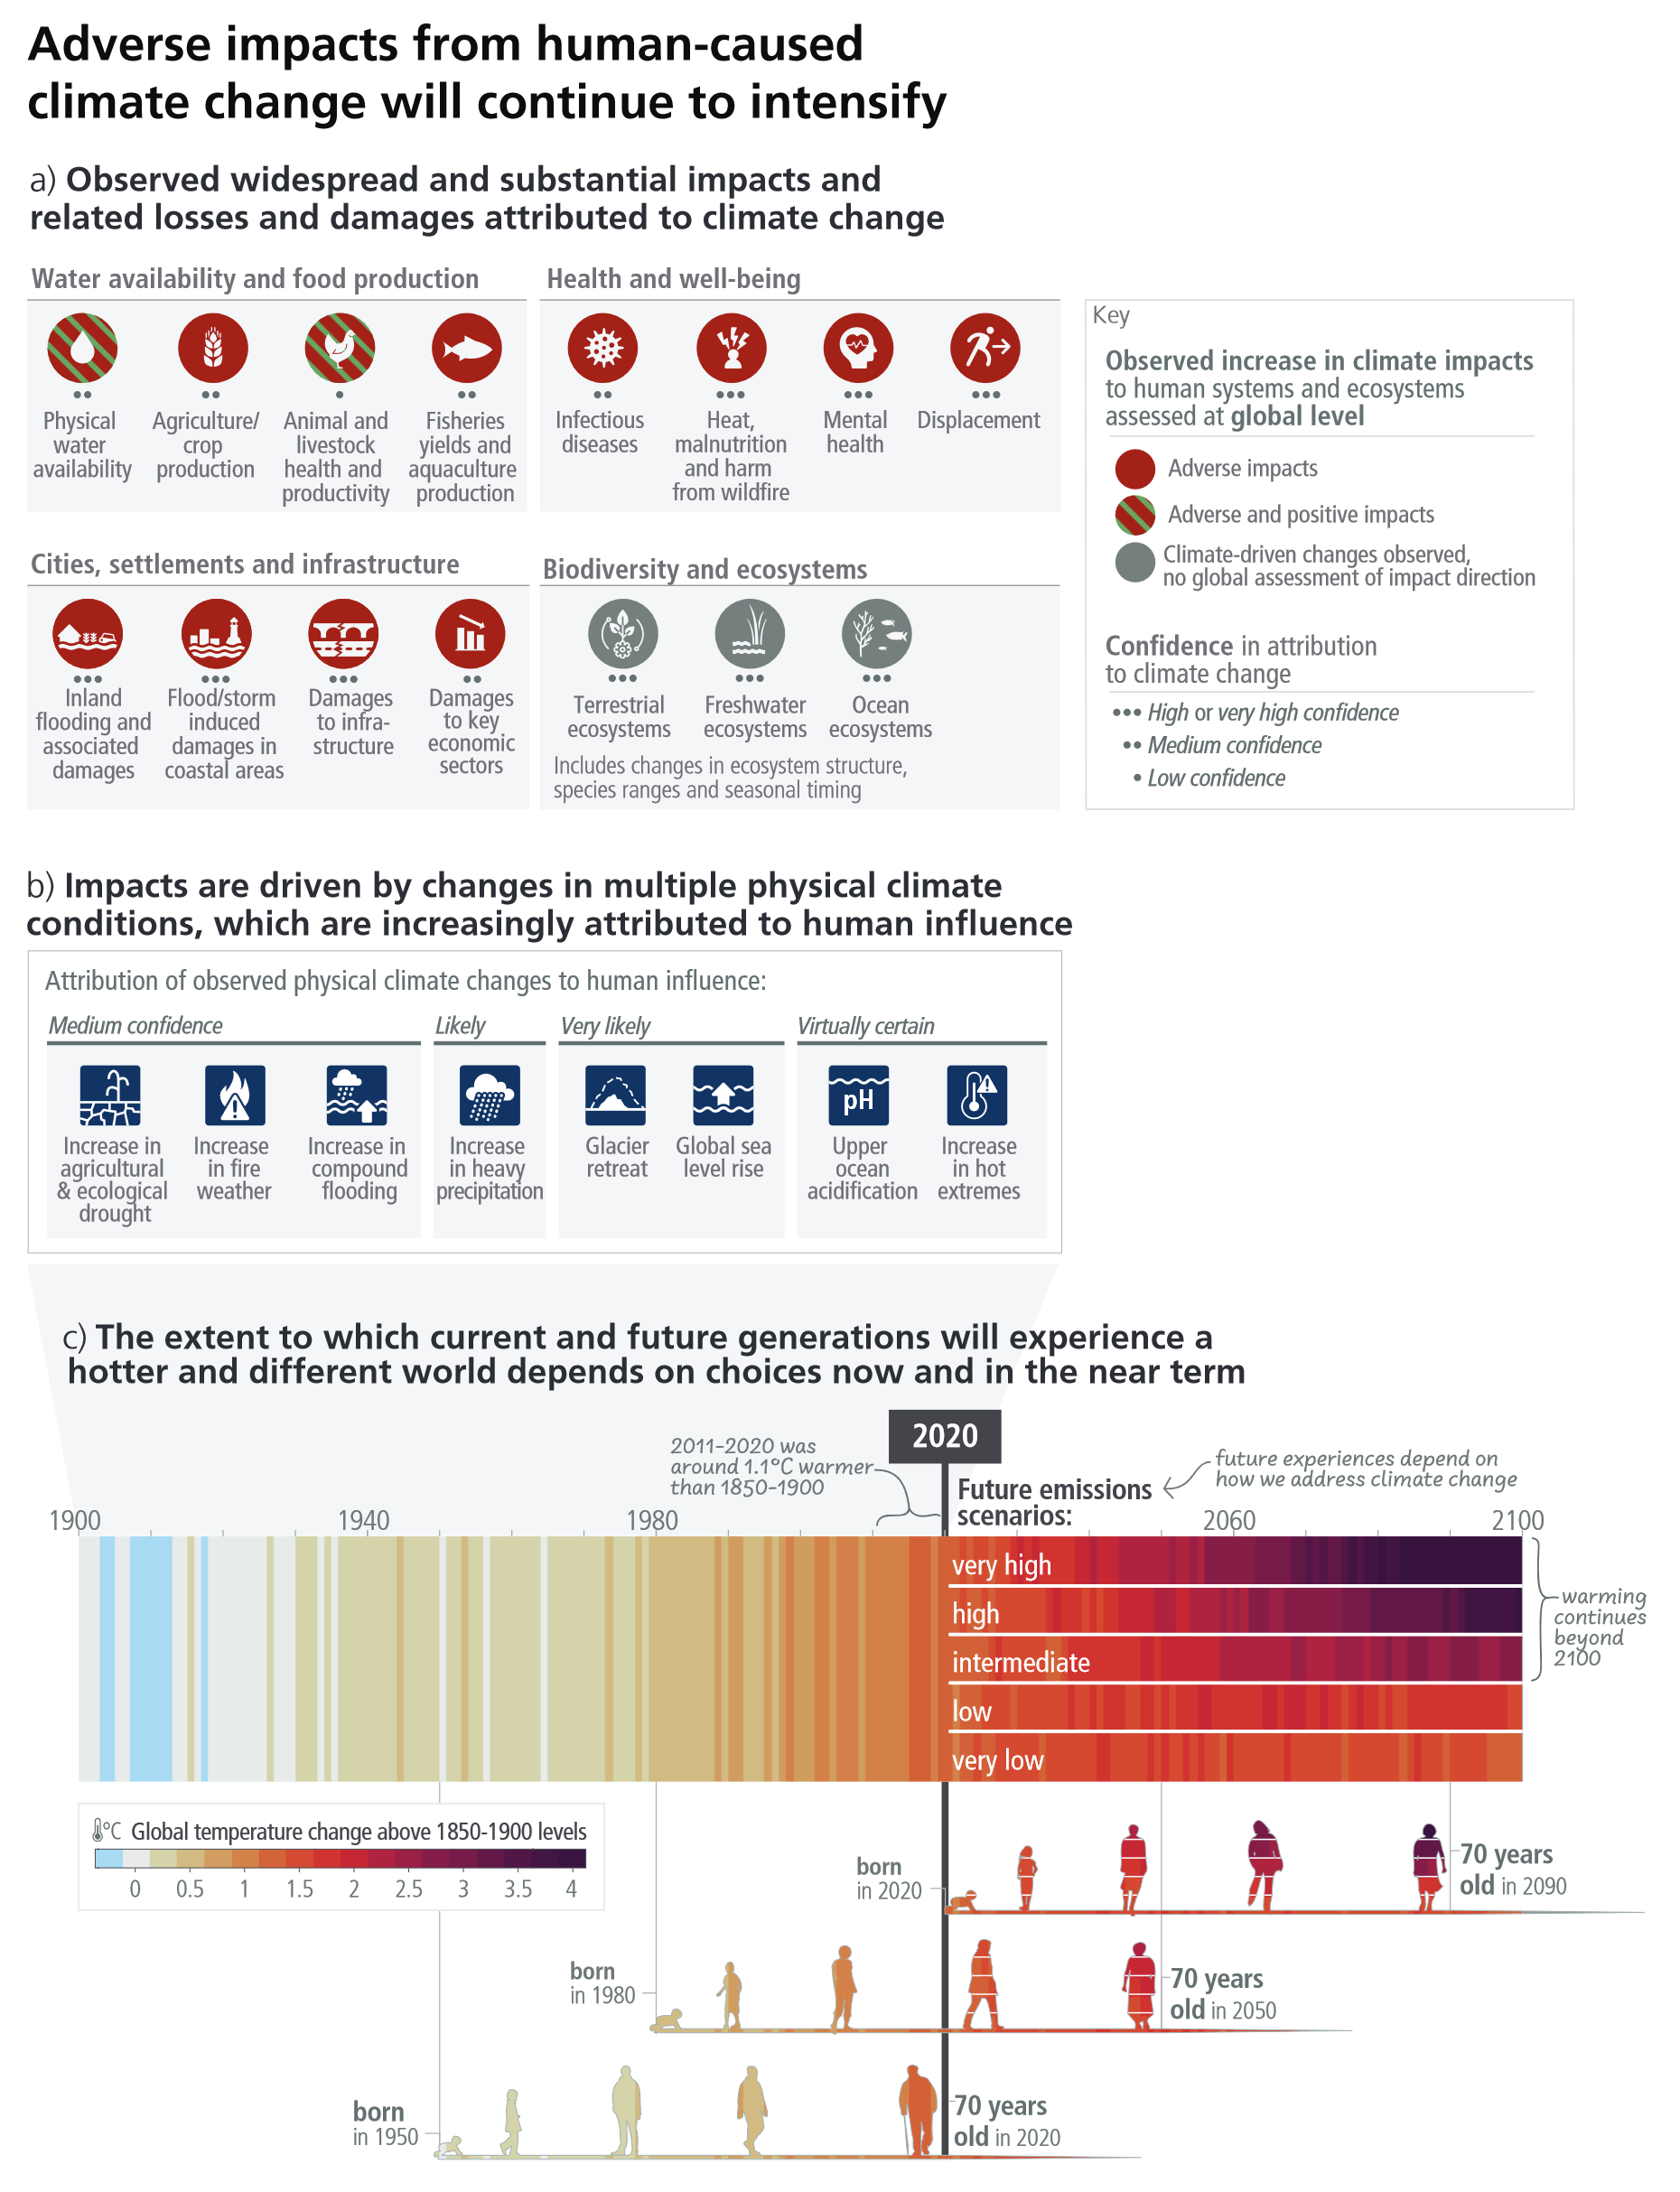
\includegraphics[width=\textwidth]{figures/spm1.png}
    \legende{Les impacts du changement climatique sont nombreux et sous des formes variées}{Les impacts du changement climatique vont continuer à s'intensifier. Ceux-ci sont regroupés en quatre catégories : eau et nourriture; santé et bien-être; villes, peuplement et infrastructures; biodiversité et écosystème (panneau a). Ces impacts sont issus de phénomènes naturels attribués à l'action humaine (panneau b). Les choix de trajectoires d'émissions impactent le niveau de réchauffement moyen, qui lui même impacte l'intensification des phénomènes. Figure issue du Synthesis Report du GIEC.}
    \label{fig:ipcc-impacts}
\end{figure}

Pour coller au mieux aux enjeux de la modélisation, nous classons ici les impacts du changement climatique en trois catégories : les effets tendanciels, qui désignent une tendance longue, dont la progression est stable et durable (augmenation du niveau de la mer, acidification des océans); les catastrophes, qui désignent des évenements soudains et de grande ampleur, souvent peu probable mais avec un impact fort (cyclones, inondations, sécheresses); enfin, on décrit les tipping points, ou points de bascule : ce sont des altérations du fonctionnement même du système, qui ne réagit plus de la même manière. 

\subsection{Les effets tendanciels}
\label{sect/1/1/1}

% Presenter les rapports du GIEC

Les effets les plus connus et souvent présentés en premier sont les effets que l'on pourrait qualifier de tendanciels. On désigne par ce terme des effets qui ont lieu de manière progressive, régulière et sur le long terme. Un exemple caractéristique est la montée du niveau de la mer. Celle-ci étant liée à la fonte des glaces et à la température des océans, elle a lieu de manière régulière au fur et à mesure que les océans se réchauffent. 



\subsection{Les catastrophes}
\label{sect/1/1/2}

A l'inverse des effets tendanciels, les catastrophes désignent des évenement soudains, ponctuels et peu probables. Ils ont la particularité d'être très mal représenté par une moyenne. Ces événements sont dans la majorité des cas non réalisés, et ont donc un niveau de dommage nul; en revanche, lorsqu'ils se réalisent, ils causent des dommages importants. Ainsi, la moyenne (ou espérance) du niveau de dommage ne capte que très mal ces phénomènes. En effet, cette moyenne serait assez faible par rapport au niveau maximal de dommage; par ailleurs, ce niveau de dommage catastrophique, lorsqu'il est atteint, peut être exacerbé par la saturation des moyens de réponse, telle que la destruction d'infrastructures critiques (routes, hopitaux) ou la surcharge de structure de réponse (services de secours, mécanismes de soutien aux populations). 

\subsection{Les tipping points}
\label{sect/1/1/3}

Enfin, les tipping points consistent en une altération profonde et durable du fonctionnement d'un système. Ayant changé de conditions, le système évolue dans une nouvelle zone, où les comportements peuvent avoir changé. Par exemple, si des conditions de sécheresse ont amené à une dégradation profonde de la flore, celle-ci ne peut plus jouer son rôle de régulateur hydrique. La disparition de ce régulateur provoque en retour des sécheresses plus importantes qu'initialement, ce qui exacerbe le phénomène. 

\begin{figure}
    \centering
    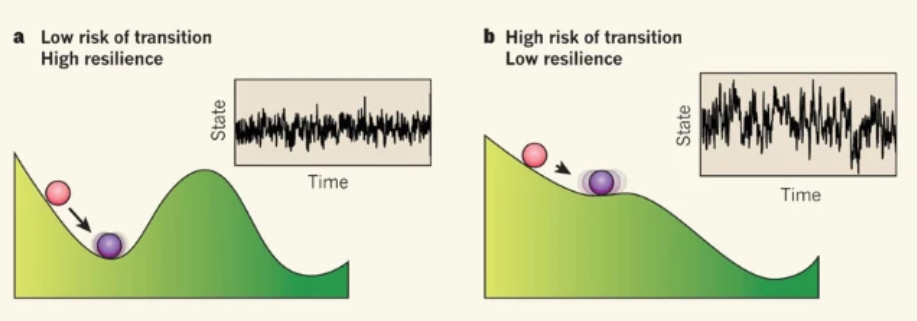
\includegraphics[width=\linewidth]{figures/tipping_point.png}
    \legende{Après un point de bascule, la dynamique du système change radicalement.}{Les tipping points, comme les événements catastrophiques, sont plus difficiles à modéliser que la tendance moyenne des dommages. }
    \label{fig:tipping-point}
\end{figure}

\begin{figure}
    \centering
    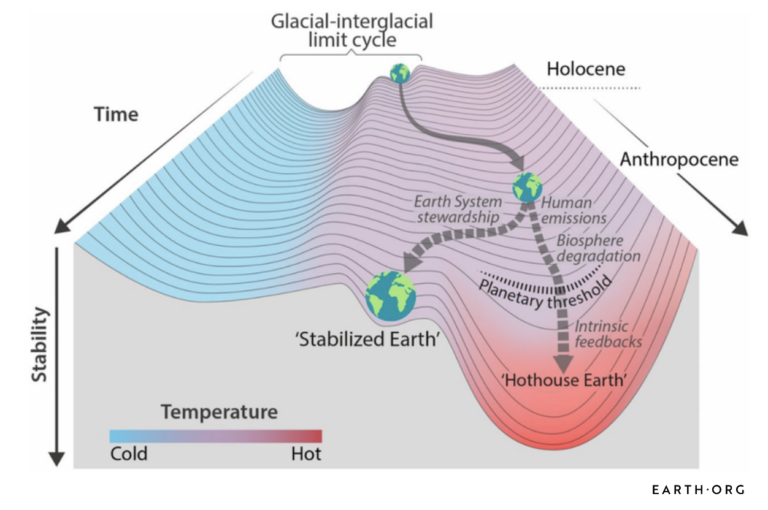
\includegraphics[width=\linewidth]{figures/earth_tipping_point.png}
    \legende{Les points de bascule dans le contexte climatique}{Les points de bascule, ou tipping points, sont des points du système où le fonctionnement de celui-ci change grandement.}
    \label{fig:earth-tipping-point}
\end{figure}

\begin{figure}
    \centering
    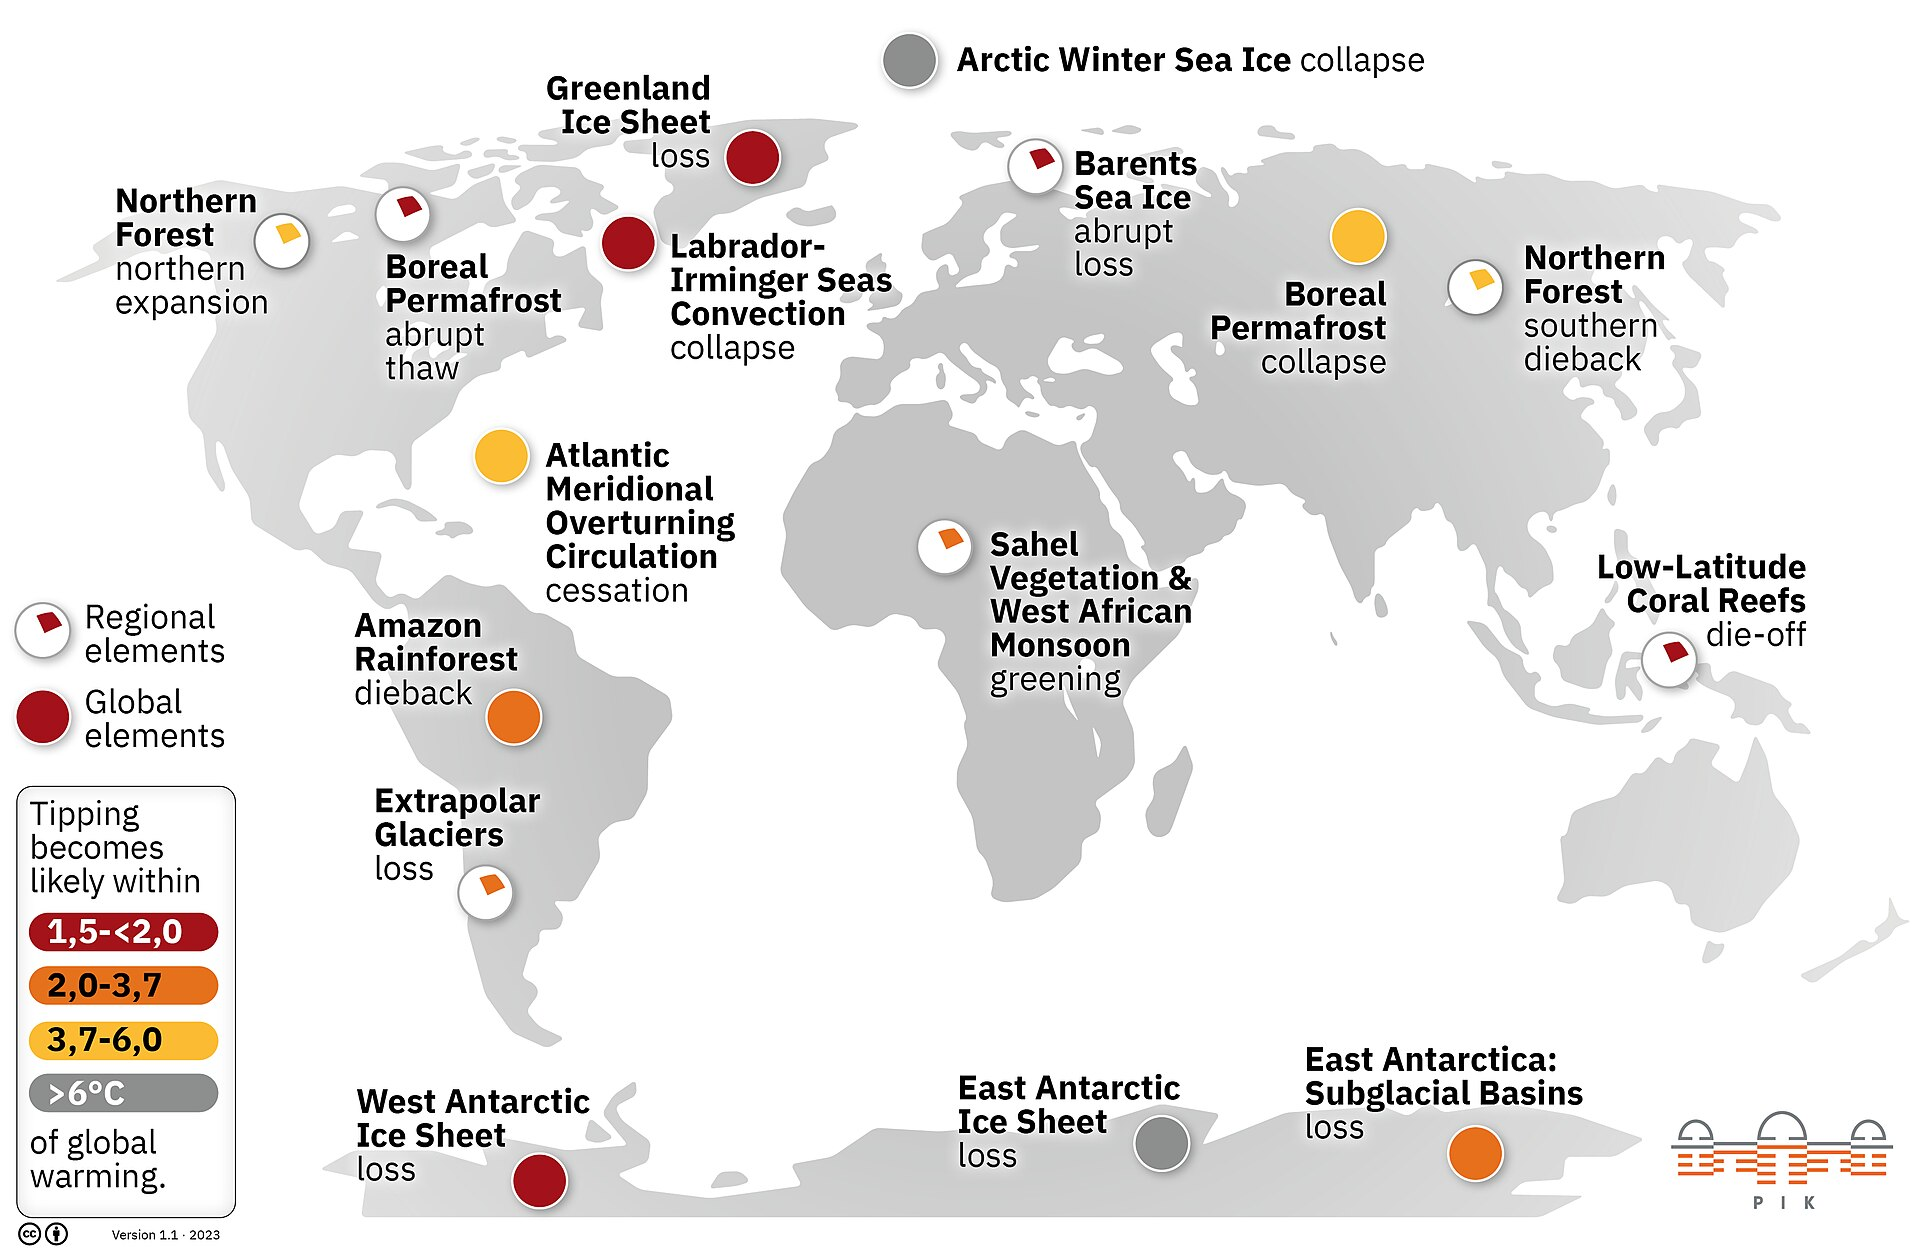
\includegraphics[width=1\linewidth]{figures/Tipping_points_2022_list.jpeg}
    \legende{Liste des points de bascule à l'échelle planétaire}{}
    \label{fig:enter-label}
\end{figure}

\paragraph{Les risk tipping points}

Au-delà de la définition classique du tipping point, l'Université des Nations Unies propose, dans son rapport sur les risques interconnectés, une nouvelle définition des risques interconnectés. Un \textit{risk tipping point}, ou point de bascule des risques, désigne \textit{l'instant où un système socioécologique ne peut plus absorber le risque et réaliser ses fonctions}. Après le passage de ce point de bascule, la possibilité d'un impact catastrophique augmente substantiellement. Six risques sont identifiés comme particulièrement représentatif des effets systémiques d'un driver sur tous les autres : l'accélération de l'extinction de la biodiversité, la réduction de l'eau de surface disponible, la fonte des glaciers, les débris spatiaux, la chaleur trop importante, et un futur qui n'est plus assurable. Parmi ces points de bascule, quatre sont  reliés à l'augmentation de la température atmosphérique ou océanique, et quatre à l'augmentation de la concentration en gaz à effet de serre dans l'atmosphère. \cite{united_nations_university_-_institute_for_environment_and_human_security_unu-ehs_interconnected_2023}

Ce concept est intéressant pour deux raisons : d'abord, il illustre la complexité des systèmes physiques et sociaux, et la complexité de leur interaction. Ensuite, il montre que la prise en compte d'un impact par le moyen d'un seul mécanisme risque de sous-estimer cet impact, car cela ne permet pas de prendre en compte les réactions en chaines et les interactions entre les différents impacts. Il étend ainsi la notion de tipping point, principalement utilisé pour caractériser des aléas, dans une lecture de risque, en interaction avec des enjeux. 

\section{Prendre des décisions dans l'incertain : le rapprochement de la science et du pouvoir}
\label{sect/1/2}

Dans cette section, nous proposons un bref retour historique sur des grandes dates ayant marqué la politique climatique. Des premières identifications du changement climatique à l'avènement d'un \emph{régime climatique}, nous verrons comment les discussions autour des enjeux climatiques se sont structurés. On cherchera à présenter les grands repères, tout en montrant comment l'histoire des négociations climatiques et des modèles intégrés sont intimmement liées, et s'influencent réciproquement. Cette partie permettra donc d'introduire l'influence qu'a le contexte sur les modèles et vice-versa. 

%Ressource : gouverner le climat

\subsection{Historique des négociations climatiques}
\label{sect:1.2.1}

L'histoire des négociations climatiques s'inscrit dans une dynamique longue, qui lit intimement science et politique. Elle démarre par la mise en évidence d'un changement climatique, puis par la prise de conscience de l'ampleur de celui-ci. Viennent alors les questions sur les actions à entreprendre : il ne faut plus seulement comprendre, il faut agir pour éviter le pire. Cependant, les conséquences de telle ou telle action sont inconnues, et plus de connaissance encore est nécessaire. \\

Dès 1822, Alfred Fourrier développe la théorie de l'effet de serre, selon laquelle la chaleur émise par le soleil est emmagasinée par l'atmosphère. Cette théorie est progressivement complétée par John Tyndall (1859), Svante Arrhenius (1896) et Guy Callendar (1938). Cette première phase voir l'émergence d'une problématique nouvelle, qui est progressivement identifiée par des chercheurs. Cependant, elle est à ce stade connue uniquement au sein de la communauté académique. \\

Dans une deuxième phase, le changement climatique est progressivement précisé. La courbe de Keeling, au laboratoire de Mauna Loa (figure \ref{fig:keeling}), a permis d'identifier l'augmentation de CO2 dans l'atmosphère. Dans la même période, de nombreux rapports éclaircicent la question. Le rapport Meadows au club de Rome, appelé \emph{les limites à la croissance dans un monde fini}, propose une modélisation économique qui tient compte de l'effet de la croissance sur l'environnemnt. Le comité Jason, en 1979, a un rôle de conseil auprès du gouvernement des Etats-Unis. Un rapport dirigé par Jules Cherney en 1979 donne une première estimation de la sensibilité du climat, et donne un réchauffement moyen de 3\textdegree C. Enfin, des institutions se sont mise en place. L'organisation météorologique mondiale (OMM), qui va prendre un rôle majeur par la suite, est fondée en 1950. D'autres programme de recherche sont mis en place : le global atmospheric research program, fondé en 1967, vise à \emph{comprendre, d’observer, de simuler et de prévoir la dynamique atmosphérique, tout en acquérant les données globales nécessaires à cet objectif}. En 1969, le comité SCOPE renforce la surveillance de l'environnement au niveau mondial. 

\begin{figure}
    \centering
    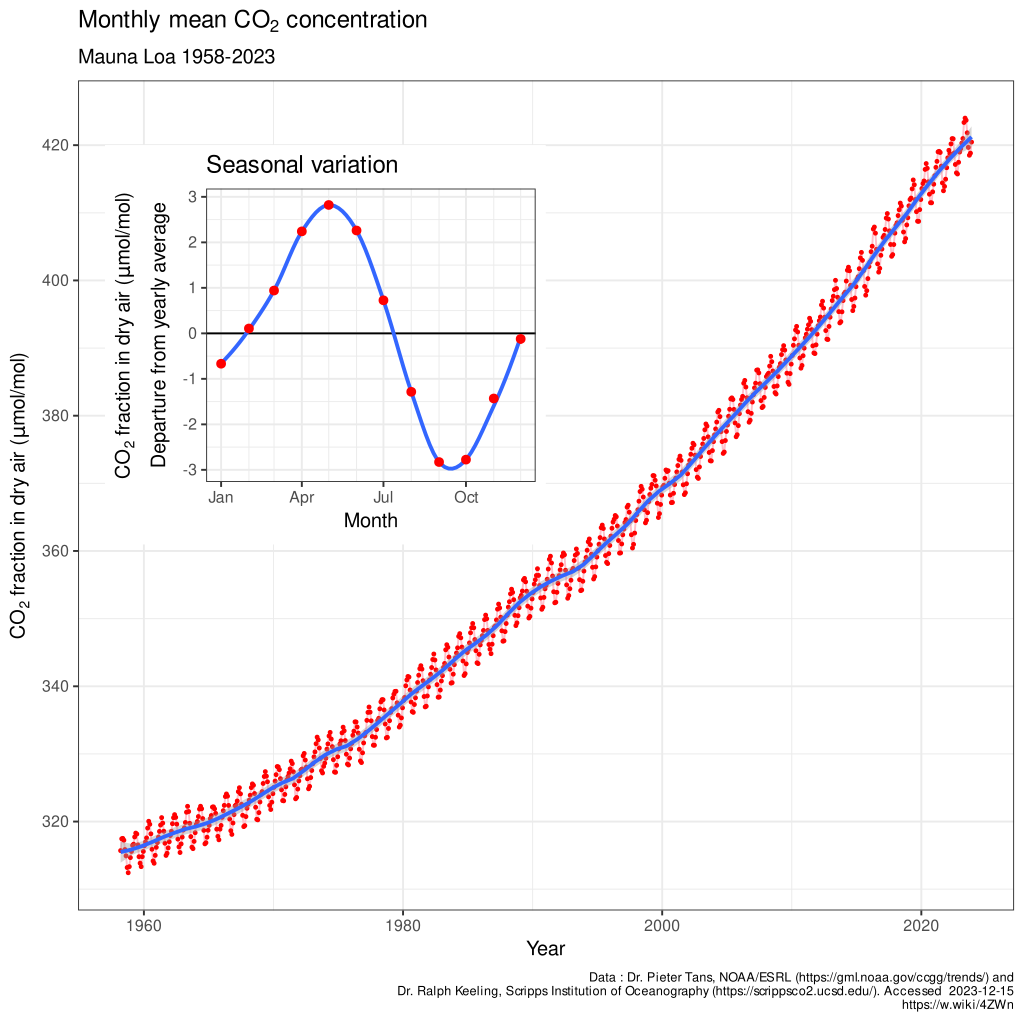
\includegraphics[width=0.5\linewidth]{figures/keeling_curve.png}
    \legende{Courbe de Keeling}{Cette courbe représente la mesure de la concentration atmosphérique de CO2 dans l'atmosphère, au niveau du laboratoire de Mauna Loa. Elle a permis d'identifier l'augmentation de la concentration de ce gaz à effet de serre dans l'atmosphère.}
    \label{fig:keeling}
\end{figure}

Une troisième phase voit ces différentes institutions se formaliser. La recherche, désormais abondante, doit être synthétisée, référencée et mise à la disposition des décideurs politiques. C'est dans cet objectif que né le GIEC en 1990, sous l'égide de l'Organisation Météorologique Mondiale et du Programme des Nations Unies pour l'Environnement (UNEP). La coopération internationale s'organise aussi. En 1992, le Sommet de la Terre de Rio s'appuie sur les conclusions du premier rapport du GIEC pour coordonner les actions des États membres du système des Nations Unies autour des questions climatiques. La Convention Cadre des Nations Unies sur le Changement Climatique est adoptée. Elle crée le système des Conference of Parties, réunion annuelles où se regroupent les états membres, ou parties à la convention, pour négocier les questions climatiques.



\begin{figure}
    \centering
    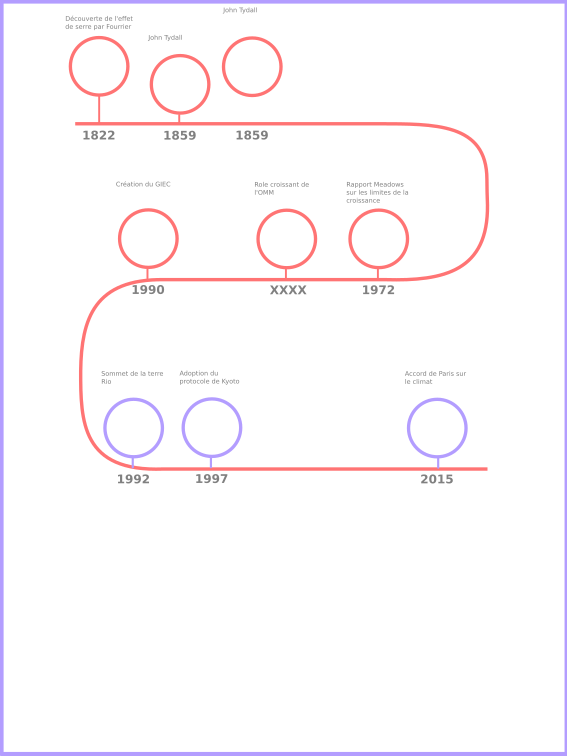
\includegraphics[width=\linewidth]{illustrations/frise.png}
    \legende{Historique des négociations climatiques}{A faire sur Inkscape + regarder chez PBL s'ils ont pas déjà des choses comme ça}
    \label{fig:frise}
\end{figure}

\subsection{Le cadre général : CCNUCC et COP}
\label{sect:1.2.2}


La Convention Cadre des Nations Unies sur le Changement Climatique (CCNUCC, ou en anglais UNFCCC), est la convention qui régit le fonctionnement des négociations internationales autour des questions climatiques. Son rôle est d'instaurer un cadre de discussion, des instances et des rendez-vous réguliers. \\

Les rendez-vous réguliers sont principalement les Conference Of Parties (COP), où se réunissent les parties à la Convention. En réalité, ces événements abritent simultanément les COP (Convention), les CMA (pour l'accord de Paris) et les CMP (pour le protocole de Kyoto). Au sein de ces conférences, les parties se regroupent en groupes de négociations, dont les intérêts et les vues sont plus proches. La figure \ref{fig:COP} montre la complexité de la composition des groupes, qui est le reflet des différences en termes de perception, d'enjeu et attentes relatifs aux sujets climatiques. \\

\begin{figure}
    \centering
    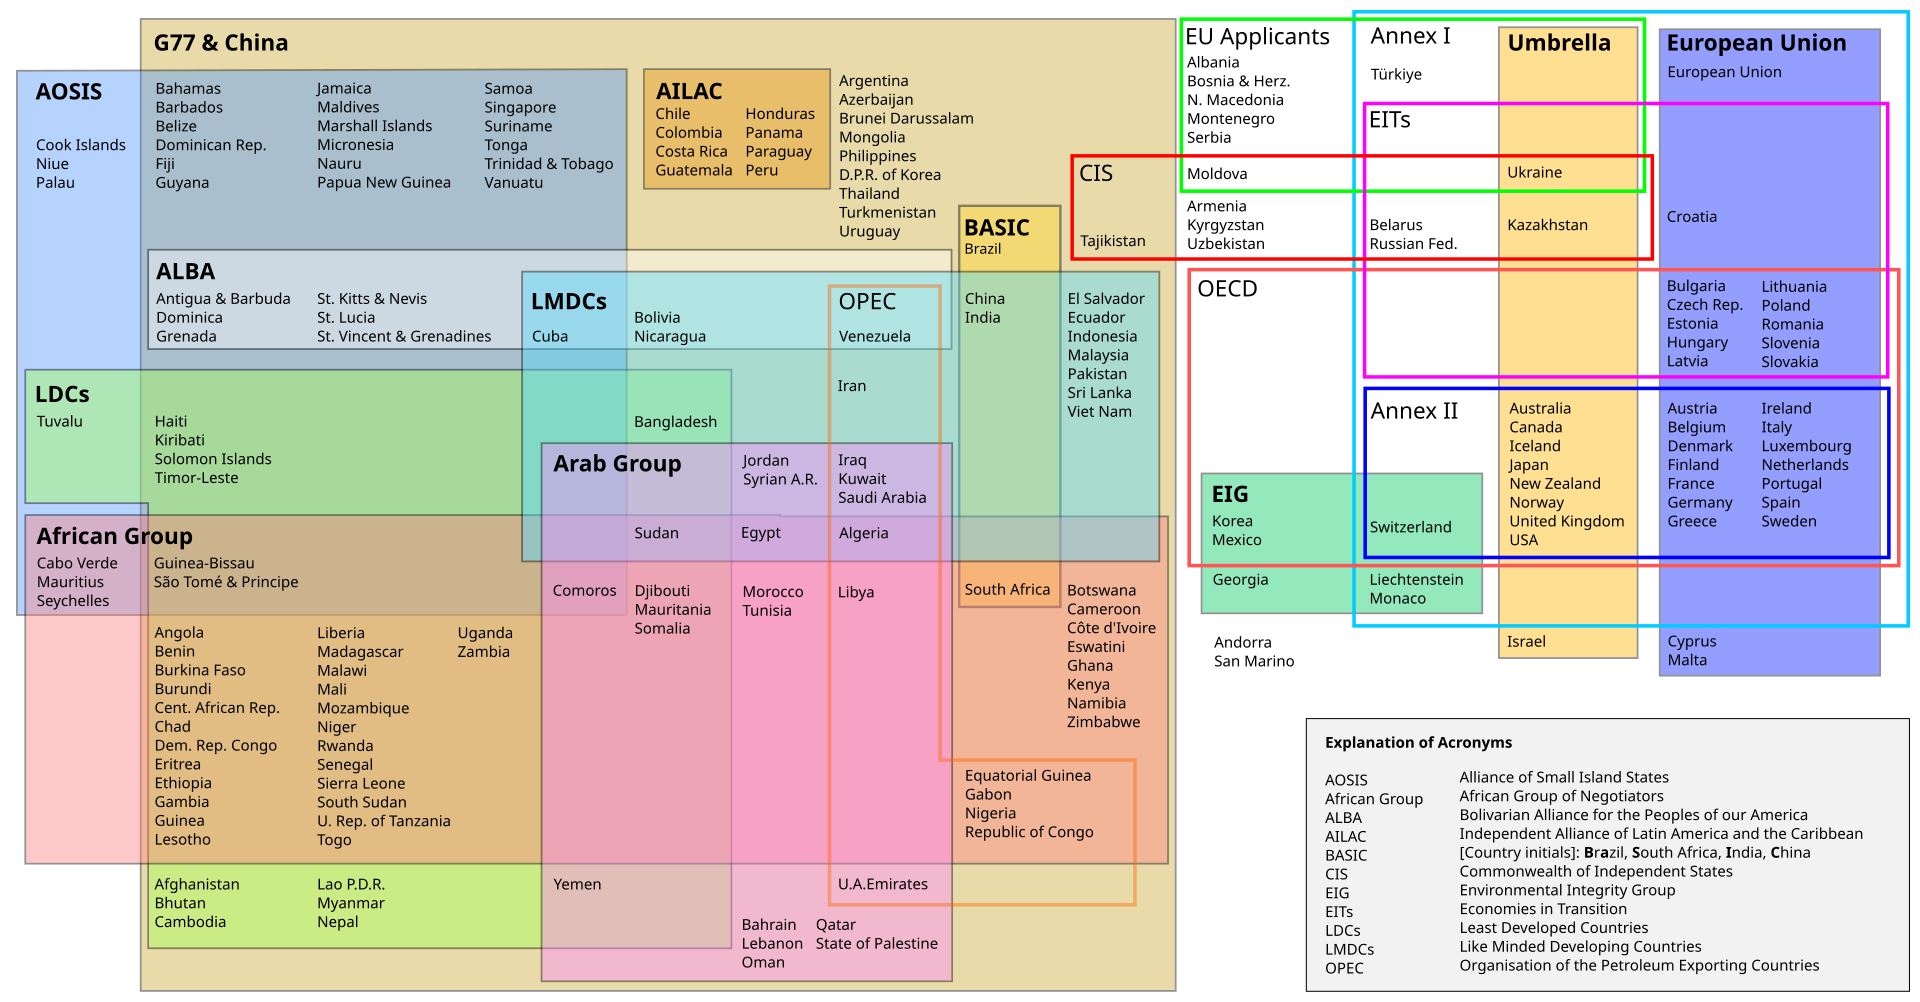
\includegraphics[width=1\linewidth]{figures/UNFCCC_Party_Groupings.svg.png}
    \legende{Groupes de négociations au sein des COP}{Les parties à la Convention cadre se regroupent selon différents groupes. \href{https://commons.wikimedia.org/w/index.php?curid=73446408}{By Jonas A. Haller - Own work, CC BY-SA 4.0}}
    \label{fig:COP}
\end{figure}

Une instance est particulièrement intéressante dans notre cas : le Subsidiary Body on Science and Technical Advice (SBSTA). Il a un rôle de tampon entre le GIEC, instance scientifique chargé de rapporter de la manière la plus fidèle et neutre possible l'ensemble des connaissances disponibles sur le changement climatique, et les parties à la Convention. Son rôle est donc à la fois scientifique et politique, et rompt avec la volonté de neutralité du GIEC. Ainsi que le présentent \cite{aykut_gouverner_nodate}, elle \emph{examine les questions scientifiques et techniques, assume l’expression politique des controverses apparues au sein des COP sur ces dernières et fait le lien entre le GIEC et les gouvernements}. Ce rôle est différent et complémentaire de celui du GIEC : il s'agit de formuler un \emph{avis}, et donc d'être plus prescriptif, tandis que le GIEC revendique de ne pas être prescriptif.  \\




\subsection{La synthèse des connaissances actuelles : le GIEC}
\label{sect:1.2.3}

Fondé en 1990, le GIEC a un mandat très clair : faire, de la manière la plus complète et rigoureuse possible, la synthèse de toutes les connaissances relatives à l'évolution du climat, en identifiant le degré de certitude de chacune de ses connaissances. Ses destinataires sont doubles : d'une part, les scientifiques eux-même, à qui il permet d'avoir une meilleure vue d'ensemble d'un champ extrememnt vaste et grandissant. D'autre part, aux décideurs politiques, leur permettant d'avoir accès de manière contextualisé à une information scientifique fiable. \\

Ainsi, le maître-mot est d'avoir une recherche qui soit \emph{policy-relevant}, mais pas \emph{policy-prescriptive} : le but est que les rapports donnent les informations nécessaires à la réalisation de politiques climatiques, sans pour autant se prononcer sur la nature ou la pertinence de ces politiques. \\

Le groupe est divisé en trois groupes de travail (Working Group - WG)  : le WG1 traite de la dimension physique du changement climatique; le WG2 traite des impacts du changement climatique et de l'adaptation, c'est-à-dire la manière de réduire les impacts du changement climatique; le WG3 traite de l'atténuation, c'est-à-dire de la manière de limiter le changement climatique lui-même. 


\subsection{Loss and damages : dommages, responsabilité et évaluation}
\label{sect:1.2.4}

TODO

\section{Les outils : de la modélisation intégrée}
\label{sect:1.3}

Les \Gls{iam} sont au coeur de l'évaluation des relations entre le climat et l'économie. Le GIEC en donne la définition suivante : \emph{{simplified representations of complex physical and social systems, focusing on the interaction between economy, society and the environment}\footnote{Représentations simplifiées de systèmes sociaux ou physiques complexes, centrés sur l'interaction entre économie, société et environnement.}}\\

Comme le souligne \cite{cointe_organising_2019}, le terme de modèle intégré désigne des choses variées. Plusieurs points caractérisent néanmoins ces modèles : ils ont une finalité de politique publique (\emph{policy-relevance}); ils sont interdisciplinaires; produisent des scénarios similaires; s'appellent spontanément modèles intégrés (IAMs); servent à évaluer les options de politique climatique. \\

La caractéristique principale des modèles intégrés est donc d'être un outil d'aide à la décision. 

On distingue généralement deux types de modèles : les modèles d'optimisation et les modèles de simulation.  
Nordhaus \cite{nordhaus_dice_2013} propose de les classer en deux catégories. D'une part, les modèles d'optimisation (\emph{policy optimization}). Il s'agit de modèles d'optimisation : ils cherchent à minimiser une variable sous contrainte d'autres variables. Concrètement, un ensemble d'équation contraint le système. Par exemple, la surface agricole est limitée par la surface disponible; le nombre de voitures électriques est limité par les réserves de lithium, etc. Ces contraintes dessinent un ensemble de mondes possibles, qui sont autant de choix disponibles et de chemins à suivre. Le modèle choisit alors un de ces chemins, qui est celui qui aura minimisé la fonction objectif (par exemple, minimisé le coût total du changement climatique, c'est à dire la somme des dommages et des investissements d'adapataion). D'autre part, les modèles d'évaluation (\emph{policy evaluation}). Ces modèles évaluent les états successifs du système, à partir d'un état initial et sur la base de relations entre les différentes variables. Ils ne permettent pas d'optimiser une issue économique ou environnementale, mais permettent de connaître l'état de chaque variable à tout moment. 
Le GIEC garde la même distinction,  \cite{intergovernmental_panel_on_climate_change_ipcc_annex_2023}, entre d'une part des modèles intégrés d'analyse coût-bénéfice (\emph{cost-benefit IAMs}), et d'autre part des \emph{process-based IAMs}.



\begin{figure}
    \centering
    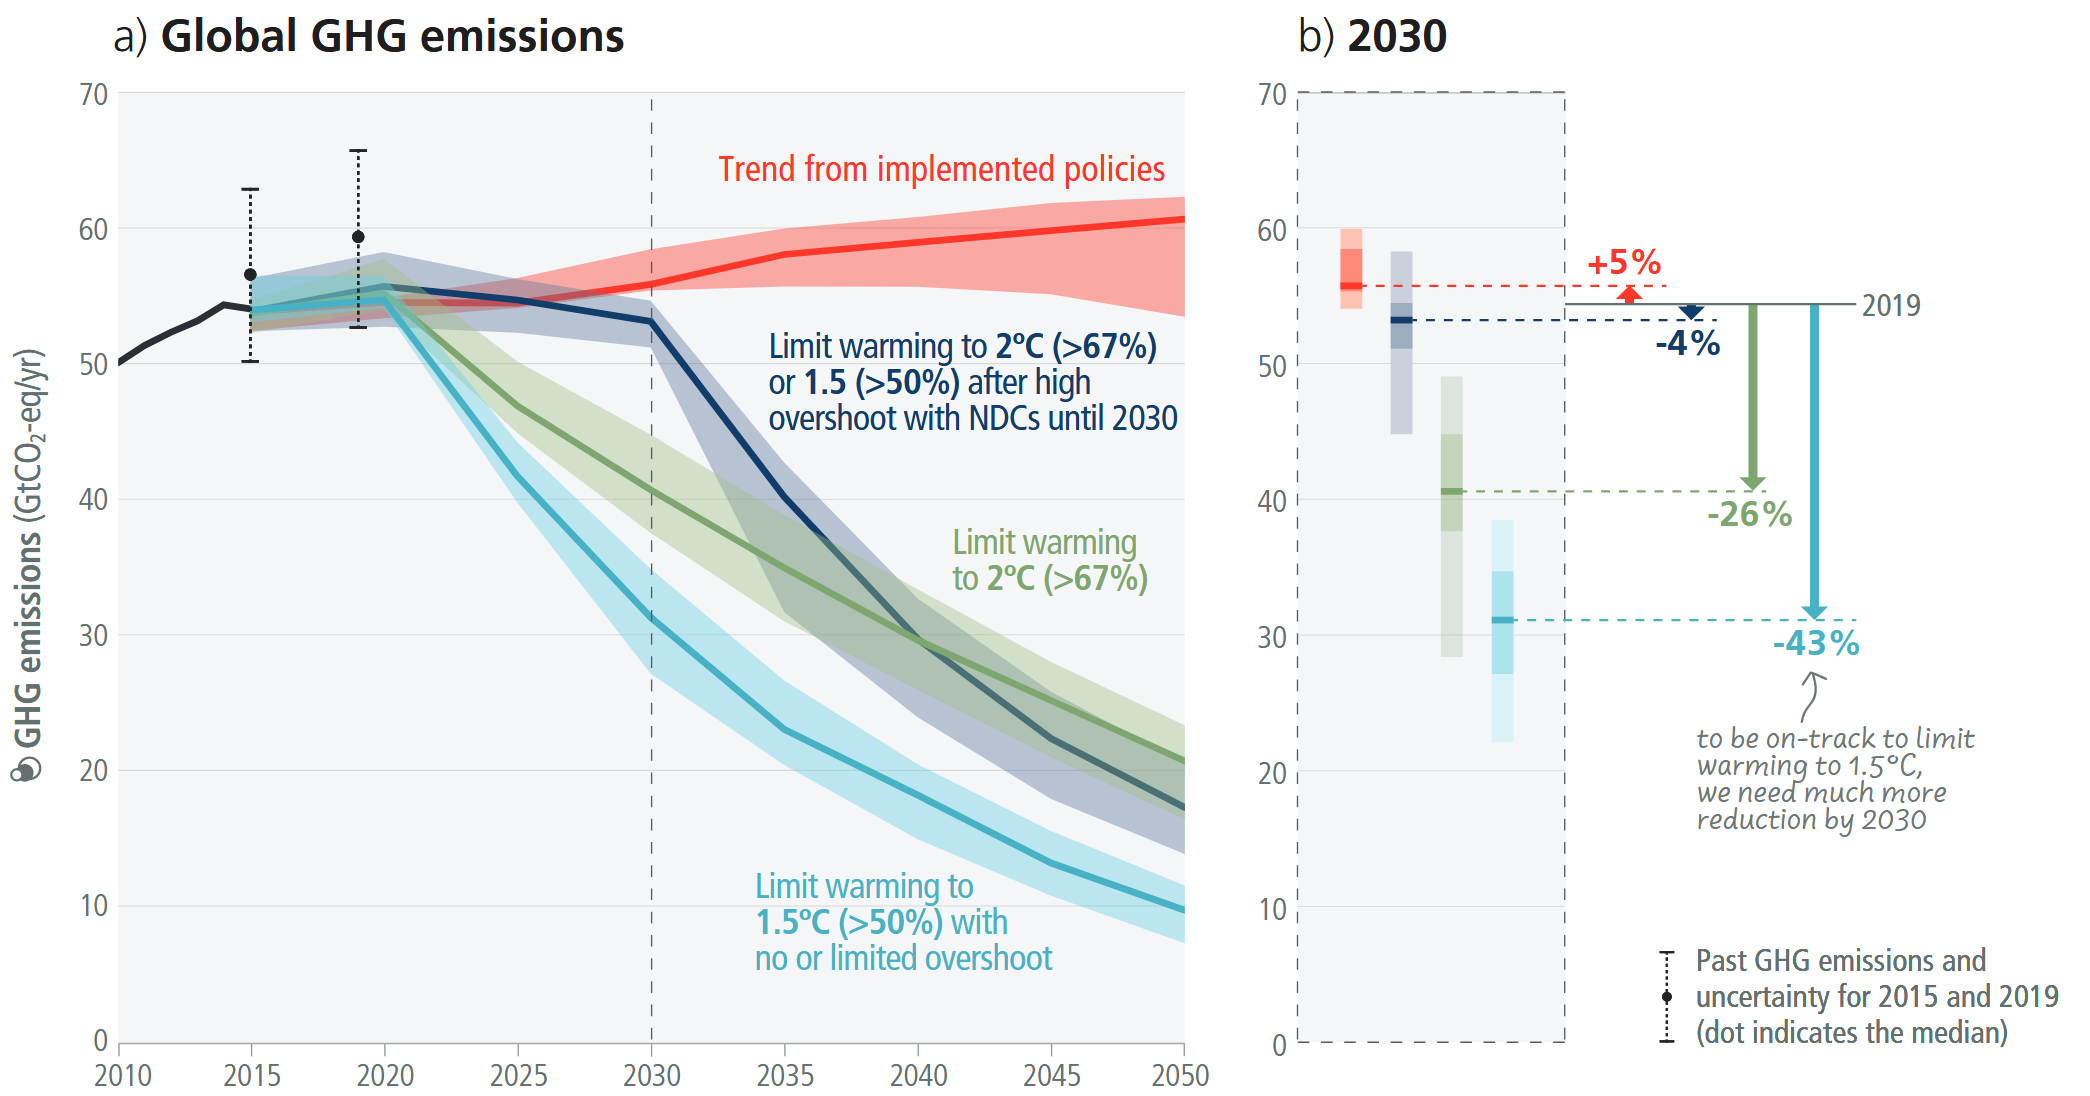
\includegraphics[width=0.9\linewidth]{figures/spm2_5.png}
    \legende{Trajectoires présentées dans le rapport de synthèse du GIEC}{Les rapports du GIEC présentent des trajectoires. Celles-ci sont obtenues à l'aide de modèles.}
    \label{fig:ipcc-pathways}
\end{figure}

De nombreuses limitations sont souvent évoquées sur les modèles intégrés. 

D'abord, la transparence.

\begin{quote}
    Unfortunately, many climate-economics models suffer from a lack of transparency, in terms of both their policy relevance and their credibility. Building a model of the climate and the economy inevitably involves numerous judgment calls; debatable judgments and untestable hypotheses turn out to be of great importance in determining the policy recommendations of climate-economics models, and should be visible for debate. \cite{stanton_inside_2009}
\end{quote}

Ensuite, la monétarisation : 

\begin{quote}
    The difficulty in fully representing the extent of climate damages in monetary terms may be the most important and challenging limitation of IAMs and it is mostly directed to costbenefit IAMs. \cite{intergovernmental_panel_on_climate_change_ipcc_annex_2023}
\end{quote}

La capacité à modéliser des phénomènes non-linéaires ou non physique interroge : pour le GIEC, \emph{there are concerns that IAMs are missing important dynamics}, ou plus précisement, 

\begin{quote}
    there are concerns that IAMs are describing transformative change on the level of energy and land use, but are largely silent about the underlying socio-cultural transitions that could imply restructuring of society and institutions
\end{quote}

Enfin, le cadrage des modèles implique de nombreux choix de modélisation fortements normatifs : 

\begin{quote}
    IAM analysis could focus on only a subset of relevant futures and thus push society in certain directions without sufficient scrutiny
\end{quote}

\subsection{Les modèles intégrés, ou comment cartographier les dynamiques du monde}
\label{sect:1.3.1}

Se baser beaucoup sur l'article de Cointe 2024 + Gouverner le climat \\

La modélisation intégrée a pris beaucoup de place au fur et à mesure que le giec a pris de l'importance

\subsection{Le coût social du carbone}
\label{sect:1.3.2}

Le coût social du carbone désigne la valorisation économique de toutes les conséquences de l'émission de carbone. Il part du principe que le coût d'utilisation des énergies carbonées (en particulier, le prix de vente de l'essence, du gaz, etc.) ne reflète pas l'ensemble des coûts qui sont causés par cette utilisation. Il y donc création d'une externalité, c'est à dire d'un impact (en l'occurence, les dommages environnementaux) qui n'est pas pris en compte lors de la transaction (en l'occurence, l'achat de carburant). Cette situation est donc suboptimale, et le surcoût est supporté par la communauté, et non par les acteurs, qui dès lors prennent une décision qui est globalement désaventageuse. Ce concept s'inscrit dans une conception économique néolibérale des échanges et dans l'analyse économique du droit.  \\

Il s'agit d'un concept utilisé principalement par les administrations des Etats-Unis, qui doivent prendre en compte cette mesure dans l'évaluation d'impact des différents projets qu'elles mettent en place. La définition donnée par l'Académie Nationale des Sciences des Etats Unis est la suivante : \emph{The social cost of carbon is « defined for a given year as the present discounted value of the future damage4 caused by a 1 metric ton increase in CO2 emissions to the atmosphere, in that year, or, equivalently, the benefits of reducing CO2 emissions by the same amount in that year. » }\footnote{Le coût social du carbone est défini pour une année donnée comme la valeur actualisée des dommages futurs causés par une tonne de CO2 émises dans l'atmosphère, ou, de manière équivalente, aux bénéfices apportés par la réduction des émissions de CO2 de la même quantité.} \\

Depuis plus de 30 ans, le coût social du carbone est calculé par un groupe de travail inter-agences fédérales qui évalue et donne une valeur chiffrée à une tonne de carbone. Des décrets présidentiels ont progressivement fixé les conditions dans lesquelles les agences doivent tenir compte de cette mesure. Désormais, toutes les agences fédérales doivent considérer l'impact en termes d’émissions de CO2 dans leurs évaluations d'impact, en tenant compte de cette valeur monétaire. \\

\begin{quote}[National Academy of Science, 2017]
     In deciding whether and how to regulate, agencies should assess all costs and benefits of available regulatory alternatives, including the alternative of not regulating. Costs and benefits shall be understood to include both quantifiable measures (to the fullest extent that these can be usefully estimated) and qualitative measures of costs and benefits that are difficult to quantify, but nevertheless essential to consider. Further, in choosing among alternative regulatory approaches, agencies should select those approaches that maximize net benefits. 
\end{quote}

Les valeurs du SCC sont calculées par le groupe de travail inter-agences sur le coût social du carbone. Pour ce faire, le groupe de travail utilise trois modèles (FUND, DICE et PAGE) et exécute des simulations en faisant varier aléatoirement les paramètres. La valeur qui est conservée est la moyenne de l'ensemble des simulations. 

\begin{figure}
    \centering
    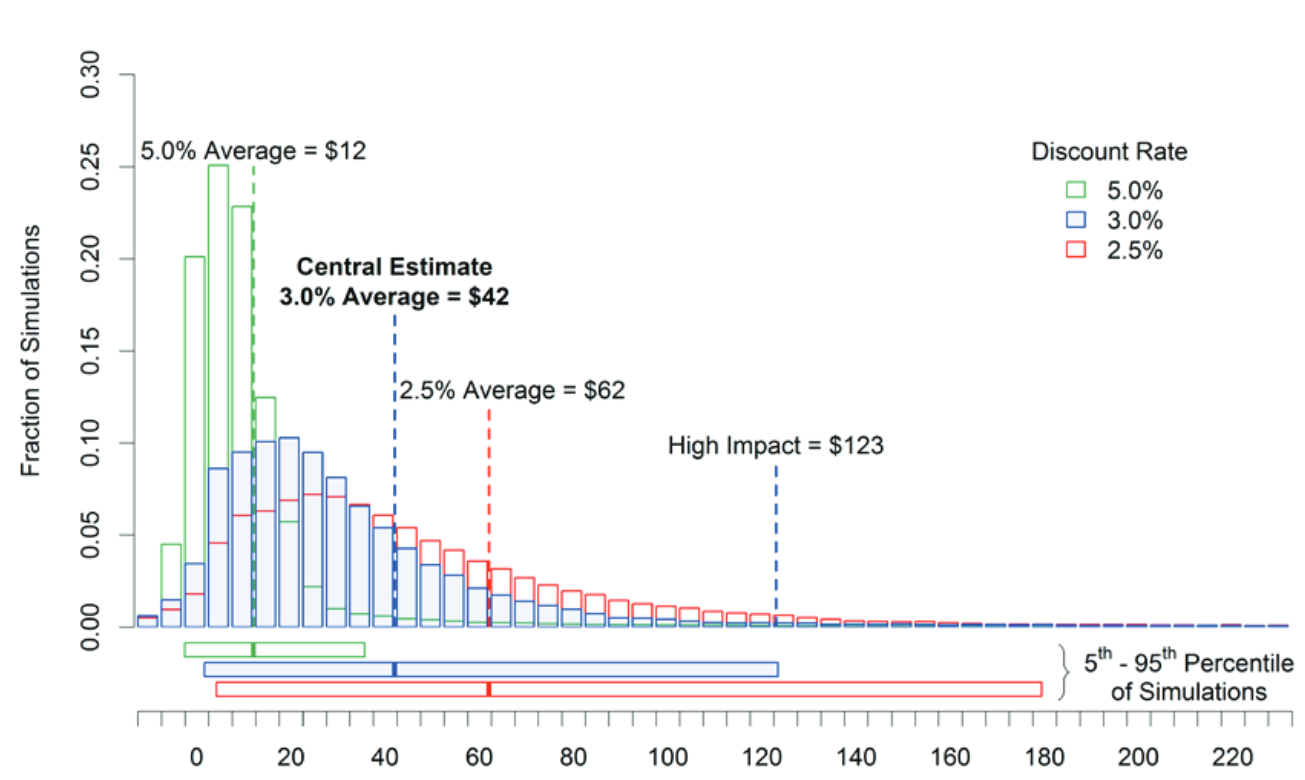
\includegraphics[width=0.9\linewidth]{figures/scc.png}
    \legende{Distribution du Coût Social du Carbone selon le taux d'actualisation (en \$/T $CO_2$)}{Le groupe de travail inter-agences pour le coût social du carbone réalise de nombreuses simulations à partir des modèles FUND, DICE et PAGE. Chaque simulation abouti à une estimation du SCC, dont les distributions sont représentées ici. Elles sont séparées par taux d'actualisation, c'est à dire la valeur que perdent les dommages chaque année. Plus cette valeur est importante, plus la préférence pour le présent est importante, et moins les dégâts futurs sont reflétés dans le SCC. On voit que ces valeurs varient considérablement selon le choix du taux d'actualisation. D'après \cite{national_academy_of_sciences_valuing_2017}}
    \label{fig:scc}
\end{figure}

\subsubsection{Historique du concept}

Le coût social du carbone 

\subsubsection{Intérêt}

\subsubsection{Critiques}




\begin{figure}
    \centering
    %\includegraphics{}
    \legende{Estimation des coûts sociaux du carbone par le groupe inter-agence}{Depuis 30 ans, les agences fédérales des États-Unis doivent inclure le coût social du carbone dans leurs études d'impact. Celui-ci est estimé à partir de trois modèles intégrés : RICE, FUND et PAGE. Sa valeur est très sensible du taux d'actualisation.}
    \label{fig:scc}
\end{figure}

\subsection{Les fonctions de dommage}
\label{sect:1.3.3}

\begin{figure}
    \centering
    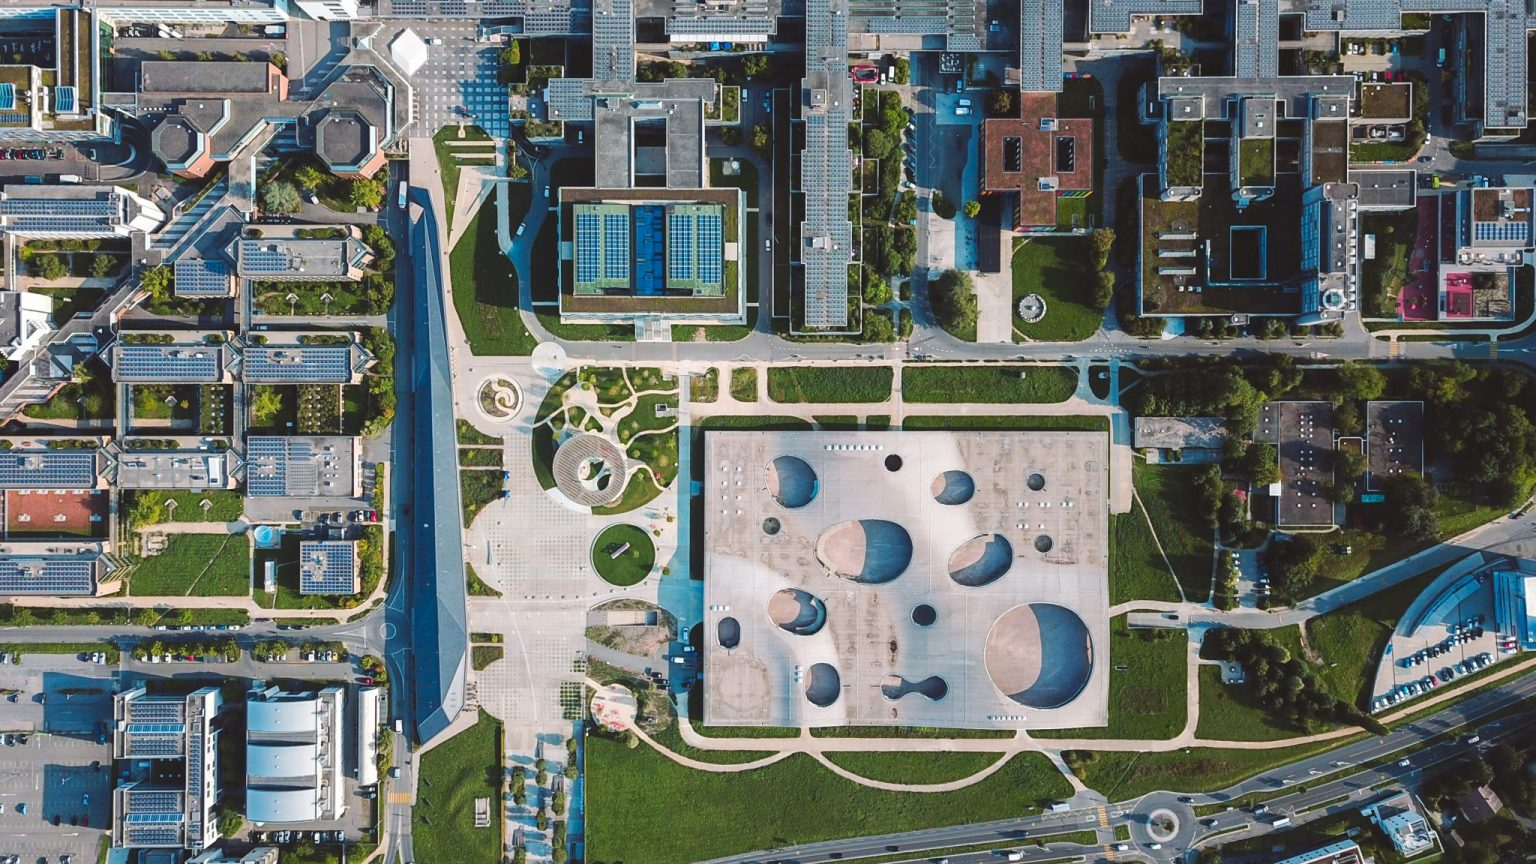
\includegraphics[width=4cm]{figures/campus.jpg}
    %\begin{tikzpicture}[scale=1]

\def\figureheight{20} % Choisis la hauteur désirée
\def\nodedistance{\textwidth*1/3}
\def\verticaldistance{2cm}
\def\nodewidth{3cm}

% Trajectory
\draw[line width = 2pt, rounded corners=8pt] (0,0) -- node[midway, below]{Les premières intuitions} (\textwidth,0) -- (\textwidth,-\figureheight*1/3) -- node[midway, below]{L'essor de la climatologie}(0,-\figureheight*1/3) -- (0,-\figureheight*2/3) -- node[midway, below]{Naissance du \textit{régime climatique}}(\textwidth,-\figureheight*2/3);


% Phase 1 : les premières intuitions


\node (1822) at (0,0.5) {1822};
\node (fourrier) [rectangle, draw, above of = 1822, text width=\nodewidth, text centered, yshift=2cm]{
Fourrier théorise l'effet de serre \\
\includegraphics[width=\linewidth]{images/Fourier2.jpg}
};

\node (1859) [right of = 1822, node distance = \nodedistance] {1859};
\node (tyndall) [rectangle, draw, above of=1859, text width=\nodewidth, text centered]{John Tyndall};

\node (1896) [right of = 1859, node distance = \nodedistance] {1896};
\node (farrhenius) [rectangle, draw, above of=1896, text width=\nodewidth, text centered]{Svante Arrhenius};

\node (1938) [right of = 1896, node distance = \nodedistance] {1938};
\node (callendar) [rectangle, draw, above of=1938, text width=\nodewidth, text centered]{Guy Callendar};

% 1822 : Joseph Fourrier
% 1859 : John Tyndall
% 1896 : Svante Arrhenius
% 1938 : Guy Callendar


% Phase 2 : l'essor de la climatologie

% Phase 3 : l'essor du régime climatique


% Information boxes
\draw[fill=blue!20] (0.5,-1) rectangle (2.5,-2);
\node at (1.5,-1.5) {Création du GIEC};
\draw[fill=green!20] (7.5,-1) rectangle (9.5,-2);
\node at (8.5,-1.5) {Première COP};
% Add more information boxes as needed
\end{tikzpicture}
    \legende{Évolution jointe de la modélisation et des négociations climatiques.}{Les modèles climatiques ont permis en premier de concevoir et de détecter le changement climatique (A). Leur essor a accompagné le cadrage de la question climatique (B), et ils sont désormais un outil de prise de décision (C).}
    \label{fig:frise}
\end{figure}

\ref{sect/1/1}


